\section{Installing and Configuring Cardano Development Tools}\label{sec:setup}
The purpose of this book is to gather all the information for developing Cardano that currently is scattered around.
What are we going to use for our project?


\begin{itemize}
    \item \textbf{A hot Wallet}: We are going to use a wallet to test our contracts, this wallet will be used to receive tADA. We'll never store our main ADA holdings in this wallet: Wallets recommended for testnet are Nami on desktop and  Vespr for mobile.
    \item \textbf{A indexer account}: Indexers are the ones that will provide us the APIs in order to interact with the chain, we won't need to run a node for testing, let's use services and projects already there like \textbf{Maestro}, let's set up an account and get the API key.
    \item \textbf{Lucid library}: Lucid is not maintained anymore as a function and has been replaced by COMING SOON, however for testing and understanding the flow of Cardano transactions it can be really useful.
    \item \textbf{tADA}: How are we going to test without having testnet ADA? let's not mess up real ADA
    \item  \textbf{IDE}: Personally I use Visual Studio Code as IDE, but any other editor is ok since we are going to 
    \item \textbf{Cardano Node:} This is NOT mandatory at all, as homework, we could try to set up a Cardano node and interact with the chain using cardano-cli (command line), however, this is something we can do in our free time, there are other hobbies out there better than this, swimming, dancing or reading a book.
\end{itemize}

\section{Hot wallets on Cardano}
When it comes to the wallet choice on Cardano the question we should ask ourselves is: Desktop or Mobile?

\begin{table}[h!]
    \caption{Current Cardano wallets available, updated in Q2 24}
    \begin{tabular}{llll}
    Wallets & Desktop & Mobile & Website                    \\
    Nami    & X       &        & https://www.namiwallet.io/ \\
    Eternl  & X       & X      & https://eternl.io/         \\
    Begin   &         & X      & https://begin.is/          \\
    Vespr   &         & X      & https://vespr.xyz/         \\
    Lace    & X       &        & https://www.lace.io/       \\
    NuFi    & X       &        & https://nu.fi/             \\
    Yoroi   & X       & X      & https://yoroi-wallet.com/  \\
    Flint   & X       & X      & https://flint-wallet.com/  \\
    Gero    & X       &        & https://www.gerowallet.io/ \\
    Typhon  & X       &        & https://typhonwallet.io/   \\
    \end{tabular}
\end{table}

Test the wallet you like most and pick the one that gives you more user-friendly vibes for your use, a developer may require a very detailed wallet, however, a basic user may need just some very simple buttons without details.

\section{Setting Up and Connecting to Cardano Testnet}
So let's install a wallet and config for testnet 

In this example, we'll install the Nami wallet that we can find \href{https://www.namiwallet.io/}{here}

Once we install the wallet we'll get 24 seed phrase words

\begin{remark}
Never share the seedphrase or store it on a cloud, use paper or different ways to store it, software can keep track of your seedphrase and you could lose the funds.
\end{remark}

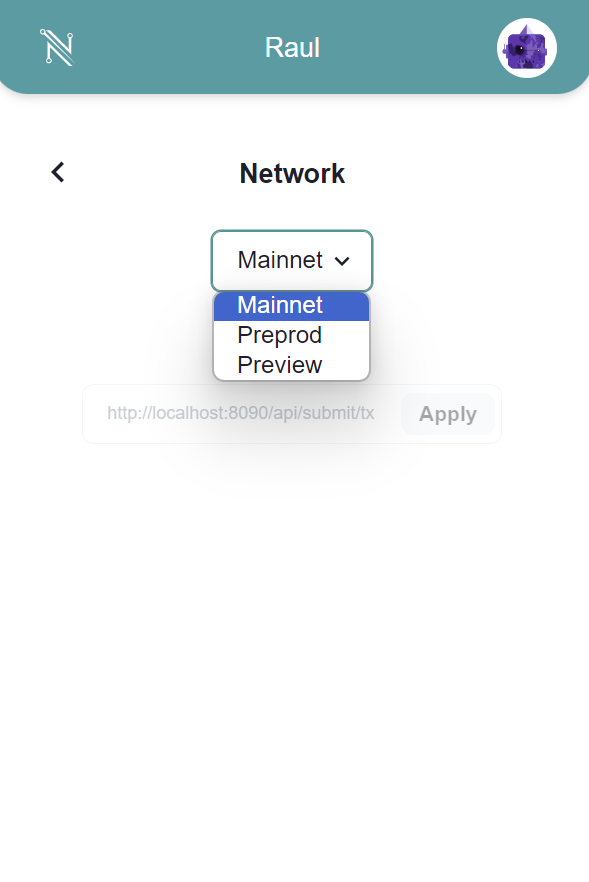
\includegraphics{wallet_preview}

Let's set Nami to \textbf{testnet preview} and we'll finally get our wallet in testnet 

\subsection{Preview and Preprod testnets}

\begin{itemize}
    \item \textbf{Mainnet}: This is the live network where real transactions occur using actual ADA. It's the primary arena where users engage with Cardano wallets, exchanges, and decentralized applications (dApps).
    \item \textbf{Preprod}: Acting as a staging ground for major upgrades and releases, Preprod is a testing environment where developers validate changes before deploying them to the mainnet. Utilizing test ADA acquired from the faucet, developers simulate real-world scenarios, ensuring everything functions as intended before the changes go live. Preprod typically mirrors mainnet's structure, forking nearly simultaneously to ensure alignment.
    \item \textbf{Preview}: Serving as a testing environment to showcase upcoming features and functionality, Preview allows developers and users to explore and provide feedback on new developments before they reach the wider community. Like Preprod, test ADA from the faucet facilitates testing. Notably, Preview precedes mainnet hard forks by a minimum of four weeks, offering ample time for thorough evaluation and refinement based on community input.
\end{itemize}

\subsection{Get tADA}

In order to receive tADA we can use the official faucet from Cardano at the following \href{https://docs.cardano.org/cardano-testnets/tools/faucet/}{link}

The process doesn't involve any payment and at the end of your testing, ideally, you should return tADA back so other devs can work with it.

\subsection{CIP30}

To connect our wallet with any webpage we'll use \gls{CIP}30 reference, we can find the list of methods to connect and invoke the functions of the wallets at this \href{https://www.cardano-caniuse.io/}{page}

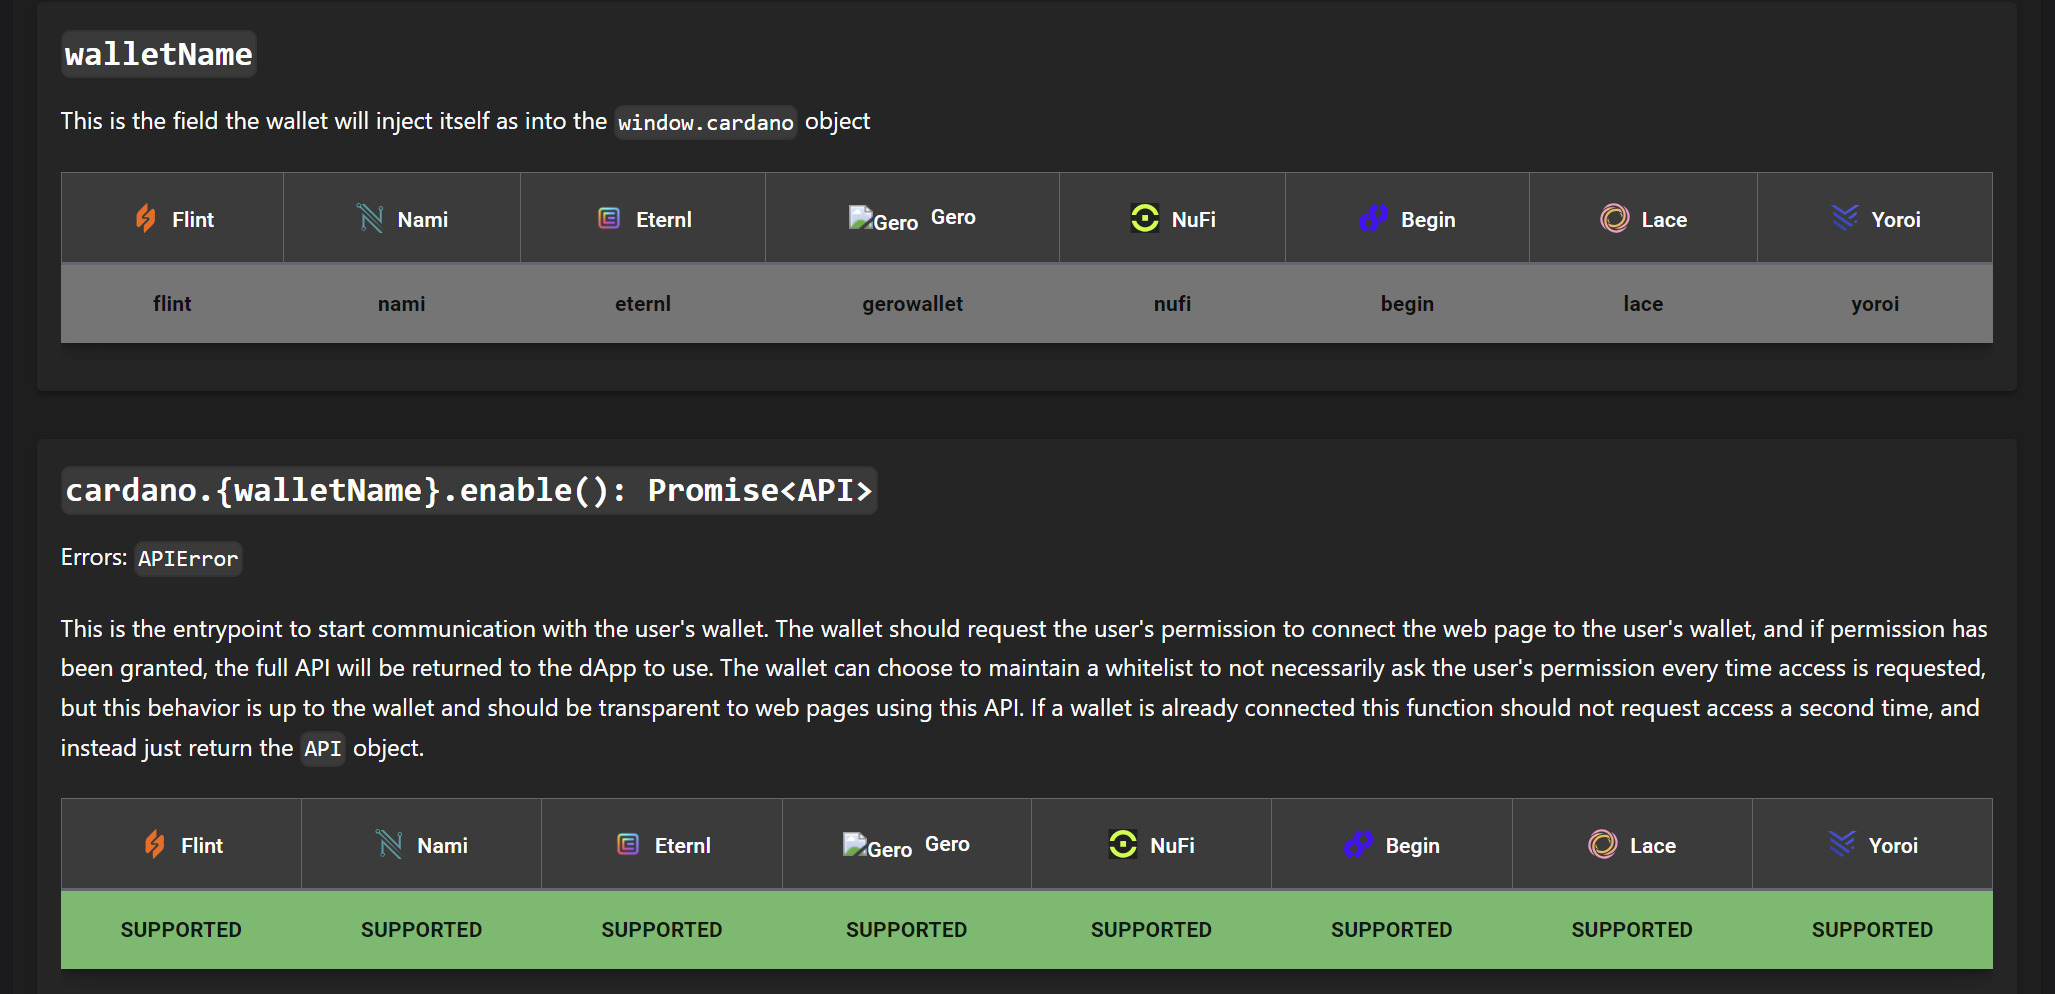
\includegraphics[scale=0.3]{cip30}

The steps to interact with a wallet following cip30 are:

\begin{itemize}
    \item \textbf{cardano.{walletName}.enable()}: we get an API object as Promise, this will create a popup message to allow the wallet to connect to the current website
    \item \textbf{api.getBalance()}: using the API object we got before, we get the total amount of Lovelace in the wallet (1 ADA = 1000,000 Lovelace)
    \item \textbf{api.signTx}: Signing a tx that was built with Lucid or any other library we sign and interact with the blockchain 
\end{itemize}

\begin{remark}
    EXERCISE 1: Create a webpage with 2 buttons, 1 to enable the wallet connection and, a second button to view the amount of ADA in the wallet.
\end{remark}




\section{Interacting with Cardano Node and Wallet APIs}

CIP30 is not enough, what if we want to get the information regarding a specific NFT in our wallet?
How to get the list of tokens inside the wallet and get information regarding their circulation supply?

We need an indexer. We could set one on our own or use a service, in this book we'll use \textbf{Maestro} as a service provider so the first thing to do is:

\subsection{Create a Maestro account}

Head over \href{https://dashboard.gomaestro.org/login}{Maestro login} page and create an account, here we'll be able to get the API keys to interact with Cardano.

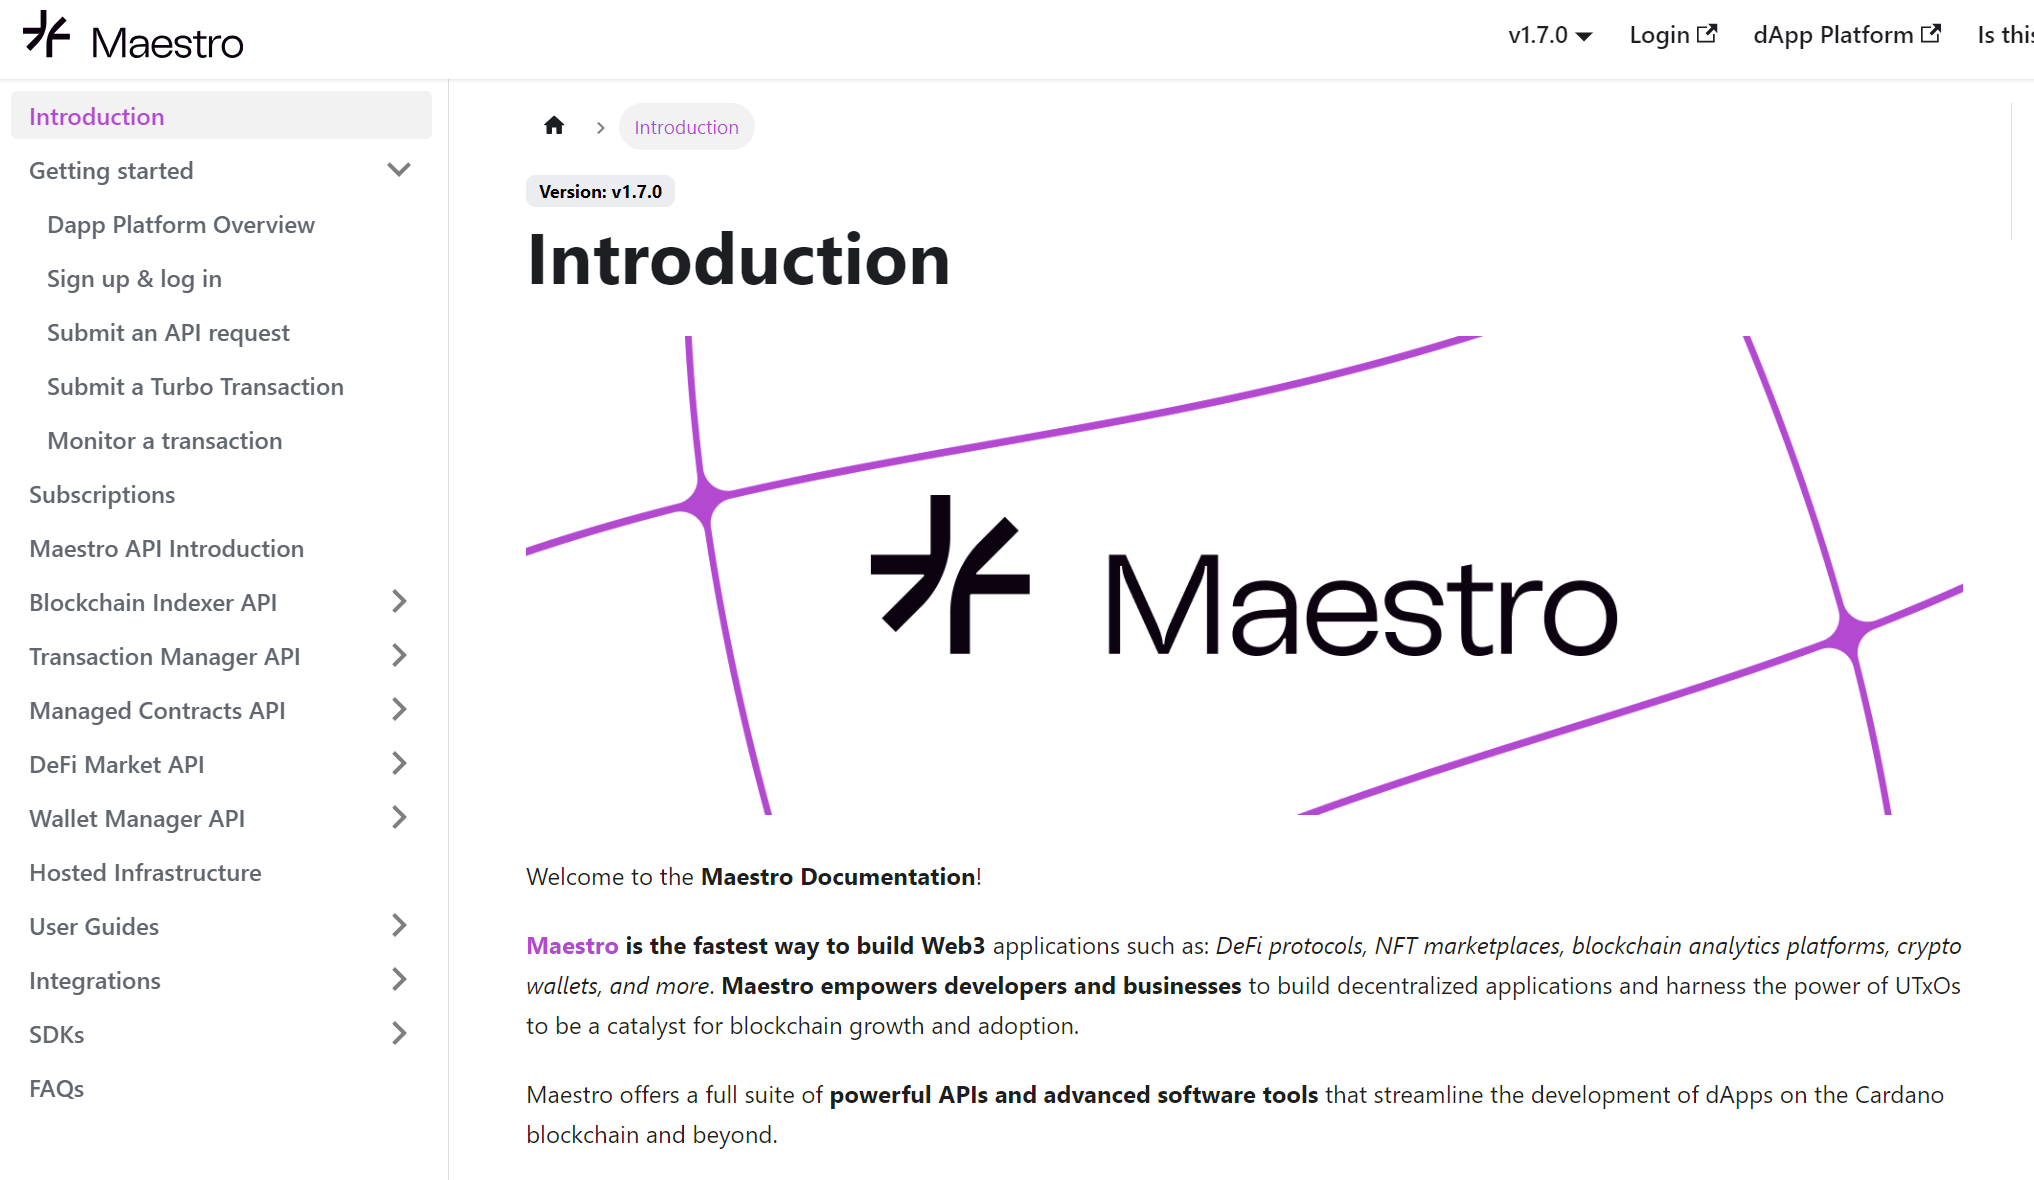
\includegraphics[scale=0.3]{maestro.png}

Maestro is going to be our key to getting all the possible APIs in order to interact with Cardano, here are the possible things we can do with these APIs:

\begin{itemize}
    \item Get the history of an address with this \href{ttps://docs.gomaestro.org/Indexer-API/Addresses/txs-by-address}{API}
    \item Get all the assets of a specific policy 
    \item Get the address holding a specific ada handle
    \item Get the history of holders for a specific NFT 
    \item and much more 
\end{itemize}

Now that we have a way to interact with a wallet and APIs to query the Cardano blockchain we are ready to put our hands on the real coding part.

\subsection{Indexer alternatives}

If you would like to explore additional API providers you should consider the following:

\begin{itemize}
    \item Blockfrost: The very first API provider for Cardano \href{https://blockfrost.io/dashboard}{link}
    \item Kupo: A tool that requires a node in order to host your own11 indexer \href{https://github.com/CardanoSolutions/kupo}{Github}
    \item Db-sync: Additional indexer that requires a Cardano Node, this is the very first one that was created \href{https://github.com/IntersectMBO/cardano-db-sync}{Github}
\end{itemize}

Now Let's code smart contracts.

\begin{remark}
    EXERCISE 2: Head over to http://cnftlab.party/ and connect your testnet wallet, mint a collection of NFTs and then use Maestro to get the information of each NFT of your collection.
\end{remark}


\section{Setting Up a Cardano Node on Contabo Cloud VPS}

\subsection{Step 1: Provisioning a Contabo Cloud VPS}
\begin{enumerate}
    \item Sign up for a Contabo Cloud VPS plan, such as the "Cloud VPS L".
    \item Once you have access to your VPS, log in via SSH.
\end{enumerate}

\subsection{Step 2: Downloading and Extracting Cardano Node Software}
\begin{enumerate}
    \item Navigate to the official Cardano GitHub release page: \href{https://github.com/input-output-hk/cardano-node/releases/tag/8.1.2}{Cardano Node Releases}.
    \item Download the Cardano Node software for macOS by running the following command:
    \begin{verbatim}
    wget https://github.com/input-output-hk/cardano-node/releases/download/8.1.2/cardano-node-8.1.2-macos.tar.gz
    \end{verbatim}
    \item After the download completes, create a directory named "node" and extract the downloaded files into it:
    \begin{verbatim}
    mkdir node
    tar xvzf cardano-node-8.1.2-macos.tar.gz -C node
    \end{verbatim}
\end{enumerate}

\subsection{Step 3: Setting Up Node Configuration}
\begin{enumerate}
    \item Create the necessary directories:
    \begin{verbatim}
    cd node
    mkdir mainnet
    cd ..
    mkdir sockets
    \end{verbatim}
    \item Create a systemd service file for the Cardano Node:
    \begin{verbatim}
    sudo nano /etc/systemd/system/cardano-node.service
    \end{verbatim}
    
    Paste the following content in the file:

    \begin{verbatim}
sudo nano /etc/systemd/system/cardano-node.service
Now we should copy and paste the following lines:
[Unit]
Description=Cardano Pool
After=multi-user.target
[Service]
Type=simple
ExecStart=/home/ubuntu/nodev30/cardano-node run --config
/home/ubuntu/nodev30/config/mainnet-config.json --topology
/home/ubuntu/nodev30/config/mainnet-topology.json --database-path
/home/ubuntu/nodev30/mainnet/db/ --socket-path  /home/ubuntu/nodev30/sockets/node.socket --
host-addr 0.0.0.0 --port 3001

KillSignal = SIGINT
RestartKillSignal = SIGINT
StandardOutput=syslog
StandardError=syslog
SyslogIdentifier=cardano
LimitNOFILE=32768

Restart=on-failure
RestartSec=15s
WorkingDirectory=~
User=USERNAMEVPS

[Install]
WantedBy=multi-user.target
    \end{verbatim}

    Save the file and exit the editor.
\end{enumerate}

\subsection{Step 4: Installing Required Dependencies and Syncing the Blockchain}
\begin{enumerate}
    \item Update package list and install necessary tools:
    \begin{verbatim}
    sudo apt update && sudo apt install liblz4-tool jq curl
    \end{verbatim}
    \item Fetch the latest blockchain snapshot and sync the blockchain:
    \begin{verbatim}
    curl -o - https://downloads.csnapshots.io/snapshots/mainnet/$(curl -s https://downloads.csnapshots.io/snapshots/mainnet/mainnet-db-snapshot.json| jq -r .[].file_name ) | lz4 -c -d - | tar -x -C /root/node/mainnet/
    \end{verbatim}
    This process may take around 30 minutes.
\end{enumerate}

\subsection{Step 5: Starting the Cardano Node}
\begin{enumerate}
    \item Enable and start the Cardano Node service:
    \begin{verbatim}
    sudo systemctl enable cardano-node.service
    sudo systemctl start cardano-node.service
    \end{verbatim}
    \item Monitor the node's status:
    \begin{verbatim}
    journalctl -u cardano-node.service -f -o cat
    \end{verbatim}
\end{enumerate}

\subsection{Step 6: Setting Up Cardano Submit API}
\begin{enumerate}
    \item Navigate to the node directory:
    \begin{verbatim}
    cd node
    \end{verbatim}
    \item Create a configuration file for the transaction submission API:
    \begin{verbatim}
    nano tx-submit-mainnet-config.yaml
    \end{verbatim}
    Paste the content from \href{https://github.com/input-output-hk/cardano-node/blob/master/cardano-submit-api/config/tx-submit-mainnet-config.yaml}{Cardano Node GitHub} into this file. Save and exit the editor.
    \item Run the Cardano Submit API with the provided configuration:
    \begin{verbatim}
    ./cardano-submit-api --tx-submit-mainnet-config.yaml --socket-path /root/node/sockets/socket node.socket --port 8090 --mainnet --host-addr 0.0.0.0
    \end{verbatim}
\end{enumerate}

\subsection{Step 7: Accessing Transaction Submission Endpoint}
With the Cardano Submit API running, you can now send transactions using your node by accessing the following URL:
\begin{verbatim}
http://VPSIPADDRESS:8090/api/submit/tx
\end{verbatim}
Replace \texttt{VPSIPADDRESS} with the IP address of your VPS.

By following these steps, you'll have successfully set up a Cardano node on your Contabo Cloud VPS and be ready to interact with the Cardano blockchain.
